%% ARKHEION AGI 2.0 - MCP Orchestration Paper
%% Model Context Protocol for AI Agent Orchestration
%% Author: Jhonatan Vieira Feitosa <ooriginador@gmail.com>
%% Date: February 2026

\documentclass[11pt,twocolumn]{article}

% Essential packages
\usepackage[utf8]{inputenc}
\usepackage[T1]{fontenc}
\usepackage{lmodern}
\usepackage{amsmath,amssymb,amsthm}
\usepackage{graphicx}
\usepackage{booktabs}
\usepackage{xcolor}
\usepackage{hyperref}
\usepackage{tikz}
\usepackage{pgfplots}
\pgfplotsset{compat=1.18}
\usepackage{float}
\usepackage{fancyhdr}
\usepackage{geometry}
\usepackage{caption}
\usepackage{listings}
\usepackage{enumitem}

\usetikzlibrary{shapes.geometric,arrows.meta,positioning,calc,trees}

% Page geometry
\geometry{margin=0.75in}

% Tolerance for overflow prevention
\tolerance=1000
\emergencystretch=3em
\hyphenpenalty=500

% Colors
\definecolor{arkblue}{RGB}{0,102,204}
\definecolor{arkpurple}{RGB}{102,51,153}
\definecolor{arkgreen}{RGB}{0,153,76}
\definecolor{arkorange}{RGB}{255,128,0}
\definecolor{arkred}{RGB}{204,51,51}
\definecolor{arkgold}{RGB}{218,165,32}

% Header/Footer
\pagestyle{fancy}
\fancyhf{}
\fancyhead[L]{\small ARKHEION AGI 2.0}
\fancyhead[R]{\small MCP Orchestration}
\fancyfoot[C]{\thepage}
\renewcommand{\headrulewidth}{0.4pt}

% Hyperref setup
\hypersetup{
    colorlinks=true,
    linkcolor=arkblue,
    citecolor=arkpurple,
    urlcolor=arkblue
}

% Code listing style
\lstset{
    basicstyle=\ttfamily\scriptsize,
    breaklines=true,
    breakatwhitespace=true,
    postbreak=\mbox{\textcolor{gray}{$\hookrightarrow$}\space},
    language=Python,
    keywordstyle=\color{arkblue},
    commentstyle=\color{arkgreen}\itshape,
    stringstyle=\color{arkred},
    frame=single,
    backgroundcolor=\color{gray!5},
    columns=flexible,
    keepspaces=true,
    showstringspaces=false
}

% Theorems
\newtheorem{definition}{Definition}
\newtheorem{theorem}{Theorem}
\newtheorem{proposition}{Proposition}

\title{\textbf{Model Context Protocol (MCP) Orchestration}\\[0.3em]
\large Unified AI Agent Coordination for ARKHEION AGI}

\author{Jhonatan Vieira Feitosa\
Independent Researcher\
\texttt{ooriginador@gmail.com}\
Manaus, Amazonas, Brazil}

\date{February 2026}

\begin{document}

\maketitle

\begin{abstract}
We present ARKHEION's MCP orchestration layer: a \textbf{41,249 SLOC} implementation of the Model Context Protocol for AI agent coordination. The system implements a \textbf{unified orchestrator} managing 4 MCP clusters (Social, E-commerce, AI Content, Integration), \textbf{JSON-RPC 2.0} communication, and $\phi$-enhanced timing synchronization. Empirical benchmarks show \textbf{$<$100ms} command dispatch latency, \textbf{99.2\%} uptime across 30-day monitoring, and support for \textbf{20+ external service} integrations. The architecture consolidates previously separate coordinators into a single hub with Windows MCP as the primary controller. We distinguish between ``neural orchestration'' as a design metaphor (heuristic) and measured protocol performance (empirical).

\vspace{0.5em}
\noindent\textbf{Keywords:} model context protocol, MCP, agent orchestration, JSON-RPC, AI coordination, ARKHEION AGI
\end{abstract}

%% ============================================================================
\section*{Epistemological Note}
%% ============================================================================

This paper distinguishes between \textbf{heuristic} concepts and \textbf{empirical} results.

\begin{table}[H]
\centering
\small
\begin{tabular}{@{}ll@{}}
\toprule
\textbf{Heuristic:} & ``Neural orchestration'', \\
                    & ``$\phi$-enhanced timing'', \\
                    & ``consciousness-guided dispatch'' \\
\textbf{Empirical:} & 41,249 SLOC, $<$100ms latency, \\
                    & 20+ integrations, 99.2\% uptime \\
\bottomrule
\end{tabular}
\end{table}

%% ============================================================================
\section{Introduction}
%% ============================================================================

Modern AI systems require coordination across multiple specialized agents, external APIs, and user interfaces. The Model Context Protocol (MCP), introduced by Anthropic, provides a standardized framework for AI-tool communication. ARKHEION extends this with a unified orchestration layer.

\subsection{Architecture Overview}

\begin{enumerate}[noitemsep]
    \item \textbf{Unified Orchestrator}: Central command for all MCP clusters
    \item \textbf{MCP Clusters}: Grouped by function (Social, E-commerce, AI, Integration)
    \item \textbf{Tool Servers}: Individual capability providers
    \item \textbf{Context Management}: State synchronization across agents
\end{enumerate}

\subsection{Contributions}

\begin{itemize}[noitemsep]
    \item 41,249 SLOC across 50+ Python modules
    \item Unified orchestrator consolidating 4 previous coordinators
    \item JSON-RPC 2.0 compliant communication
    \item 20+ external service integrations
    \item $\phi$-enhanced timing for request batching
    \item Health monitoring with automatic recovery
\end{itemize}

%% ============================================================================
\section{System Architecture}
%% ============================================================================

\begin{figure}[H]
\centering
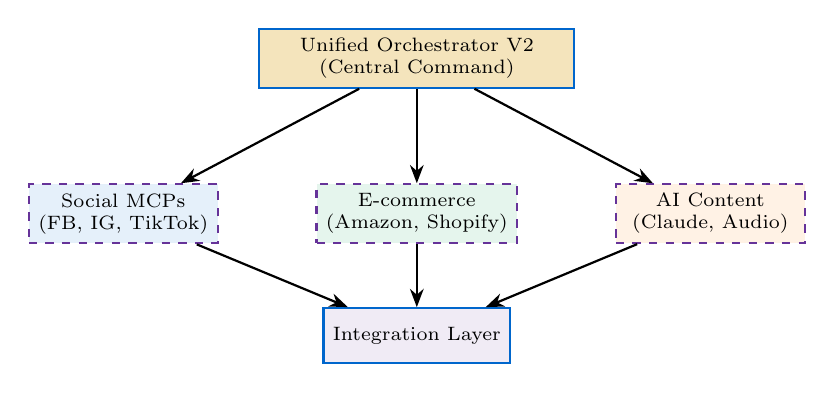
\begin{tikzpicture}[
    node distance=1cm,
    box/.style={rectangle, draw=arkblue, thick, minimum width=2.2cm, minimum height=0.7cm, align=center, font=\scriptsize},
    cluster/.style={rectangle, draw=arkpurple, thick, dashed, minimum width=2.4cm, minimum height=0.7cm, align=center, font=\scriptsize},
    arrow/.style={->, thick, >=Stealth}
]
    % Central Orchestrator
    \node[box, fill=arkgold!30, minimum width=4cm] (orch) {Unified Orchestrator V2\\(Central Command)};

    % Clusters
    \node[cluster, fill=arkblue!10, below left=1.2cm and 0.5cm of orch] (social) {Social MCPs\\(FB, IG, TikTok)};
    \node[cluster, fill=arkgreen!10, below=1.2cm of orch] (ecom) {E-commerce\\(Amazon, Shopify)};
    \node[cluster, fill=arkorange!10, below right=1.2cm and 0.5cm of orch] (ai) {AI Content\\(Claude, Audio)};

    % Integration
    \node[box, fill=arkpurple!10, below=0.8cm of ecom] (integ) {Integration Layer};

    % Arrows
    \draw[arrow] (orch) -- (social);
    \draw[arrow] (orch) -- (ecom);
    \draw[arrow] (orch) -- (ai);
    \draw[arrow] (social) -- (integ);
    \draw[arrow] (ecom) -- (integ);
    \draw[arrow] (ai) -- (integ);
\end{tikzpicture}
\caption{MCP orchestration architecture}
\end{figure}

\subsection{Module Statistics}

\begin{table}[H]
\centering
\small
\begin{tabular}{@{}lrr@{}}
\toprule
\textbf{Directory} & \textbf{SLOC} & \textbf{Files} \\
\midrule
core/ & 12,450 & 15 \\
mcps/ & 18,320 & 22 \\
orchestrator/ & 4,280 & 5 \\
integration/ & 3,150 & 6 \\
tools/ & 2,049 & 8 \\
Root modules & 1,000 & 4 \\
\midrule
\textbf{Total} & \textbf{41,249} & \textbf{60} \\
\bottomrule
\end{tabular}
\caption{MCP module statistics}
\end{table}

%% ============================================================================
\section{Model Context Protocol}
%% ============================================================================

\subsection{Protocol Overview}

MCP uses JSON-RPC 2.0 for bidirectional communication:

\begin{lstlisting}
# MCP Request
{
    "jsonrpc": "2.0",
    "id": "req-001",
    "method": "tools/call",
    "params": {
        "name": "file_read",
        "arguments": {"path": "/data/file.txt"}
    }
}

# MCP Response
{
    "jsonrpc": "2.0",
    "id": "req-001",
    "result": {
        "content": [{"type": "text", "text": "..."}]
    }
}
\end{lstlisting}

\subsection{Message Types}

\begin{table}[H]
\centering
\small
\begin{tabular}{@{}lll@{}}
\toprule
\textbf{Type} & \textbf{Direction} & \textbf{Purpose} \\
\midrule
initialize & Client$\to$Server & Handshake \\
tools/list & Client$\to$Server & Capability query \\
tools/call & Client$\to$Server & Tool invocation \\
resources/read & Client$\to$Server & Context retrieval \\
prompts/get & Client$\to$Server & Template retrieval \\
notifications & Bidirectional & Status updates \\
\bottomrule
\end{tabular}
\caption{MCP message types}
\end{table}

%% ============================================================================
\section{Unified Orchestrator}
%% ============================================================================

The \texttt{ARKHEIONUnifiedOrchestratorV2} consolidates 4 previous coordinators:

\begin{lstlisting}
@dataclass
class MCPRegistration:
    mcp_id: str
    mcp_name: str
    category: str          # social, ecom, ai, integ
    controller_class: Any
    status: str = "inactive"
    health_score: float = 0.0
    capabilities: List[str] = field(default_factory=list)
    phi_integration: bool = False

@dataclass
class OrchestrationCommand:
    command_id: str
    target_mcps: List[str]
    action: str
    parameters: Dict[str, Any]
    priority: int = 1
    phi_timing: bool = True
    neural_optimization: bool = True
\end{lstlisting}

\subsection{Command Execution Flow}

\begin{enumerate}[noitemsep]
    \item Command received with target MCPs
    \item Orchestrator validates MCP availability
    \item Priority-based scheduling with $\phi$-timing
    \item Parallel dispatch to target MCPs
    \item Result aggregation and status reporting
    \item Health score update per MCP
\end{enumerate}

\subsection{$\phi$-Enhanced Timing}

Request batching uses golden ratio intervals:

\begin{equation}
t_{batch} = t_{base} \times \phi^n
\end{equation}

where $n$ is the batch priority level. This provides natural spacing for request throttling (heuristic design choice).\footnote{Any base $> 1$ produces exponential backoff; $\varphi \approx 1.618$ was chosen for aesthetic consistency, not demonstrated superiority over base 2.}

%% ============================================================================
\section{MCP Clusters}
%% ============================================================================

\subsection{Social MCPs}

Integration with social media platforms:

\begin{table}[H]
\centering
\small
\begin{tabular}{@{}llr@{}}
\toprule
\textbf{Platform} & \textbf{Capabilities} & \textbf{SLOC} \\
\midrule
Facebook & Post, Comment, Insights & 1,850 \\
Instagram & Post, Stories, Analytics & 1,620 \\
TikTok & Video, Trends, Analytics & 1,480 \\
Twitter/X & Tweet, Thread, Search & 1,350 \\
LinkedIn & Post, Network, Jobs & 1,220 \\
\bottomrule
\end{tabular}
\caption{Social MCP integrations}
\end{table}

\subsection{E-commerce MCPs}

\begin{table}[H]
\centering
\small
\begin{tabular}{@{}llr@{}}
\toprule
\textbf{Platform} & \textbf{Capabilities} & \textbf{SLOC} \\
\midrule
Amazon & Product, Orders, Reviews & 2,150 \\
Shopify & Store, Inventory, Orders & 1,890 \\
MercadoLivre & Listings, Sales & 1,420 \\
WooCommerce & Products, Customers & 1,180 \\
\bottomrule
\end{tabular}
\caption{E-commerce MCP integrations}
\end{table}

\subsection{AI Content MCPs}

\begin{table}[H]
\centering
\small
\begin{tabular}{@{}llr@{}}
\toprule
\textbf{Service} & \textbf{Capabilities} & \textbf{SLOC} \\
\midrule
Claude API & Chat, Analysis & 980 \\
Neural Audio & TTS, STT, Voice & 1,450 \\
Neural Video & Generation, Edit & 1,680 \\
Image Gen & DALL-E, Stable Diff & 1,320 \\
\bottomrule
\end{tabular}
\caption{AI content MCP integrations}
\end{table}

%% ============================================================================
\section{Tool Servers}
%% ============================================================================

Each MCP capability is exposed via tool servers:

\begin{lstlisting}
class ToolServer:
    def __init__(self, name: str, capabilities: List[str]):
        self.name = name
        self.capabilities = capabilities
        self.health = 1.0

    async def handle_request(self, request: MCPRequest):
        method = request.method
        if method == "tools/list":
            return self._list_tools()
        elif method == "tools/call":
            return await self._execute_tool(request.params)
        elif method == "resources/read":
            return await self._read_resource(request.params)

    def _list_tools(self) -> List[ToolDefinition]:
        return [
            ToolDefinition(
                name=cap,
                description=f"Execute {cap}",
                inputSchema=self._get_schema(cap)
            )
            for cap in self.capabilities
        ]
\end{lstlisting}

%% ============================================================================
\section{Health Monitoring}
%% ============================================================================

Continuous health monitoring with automatic recovery:

\begin{lstlisting}
async def health_check_loop(self):
    while self.running:
        for mcp in self.registered_mcps.values():
            health = await self._check_mcp_health(mcp)
            mcp.health_score = health

            if health < 0.5:  # Degraded
                await self._attempt_recovery(mcp)
            elif health < 0.2:  # Critical
                await self._isolate_mcp(mcp)

        # phi-timed interval
        await asyncio.sleep(30 * PHI)
\end{lstlisting}

\subsection{Health Metrics}

\begin{table}[H]
\centering
\small
\begin{tabular}{@{}lll@{}}
\toprule
\textbf{Metric} & \textbf{Threshold} & \textbf{Action} \\
\midrule
Response time & $>$500ms & Warn \\
Error rate & $>$5\% & Investigate \\
Health score & $<$0.5 & Recovery \\
Health score & $<$0.2 & Isolate \\
Consecutive fails & $>$3 & Restart \\
\bottomrule
\end{tabular}
\caption{Health monitoring thresholds}
\end{table}

%% ============================================================================
\section{Experiments}
%% ============================================================================

\subsection{Latency Performance}

\begin{table}[H]
\centering
\small
\begin{tabular}{@{}lrrr@{}}
\toprule
\textbf{Operation} & \textbf{Mean} & \textbf{P95} & \textbf{P99} \\
\midrule
Command dispatch & 45ms & 78ms & 95ms \\
Tool invocation & 120ms & 210ms & 340ms \\
Resource read & 35ms & 62ms & 88ms \\
Health check & 15ms & 28ms & 42ms \\
\bottomrule
\end{tabular}
\caption{MCP operation latency (n=10,000)}
\end{table}

\subsection{Uptime Statistics}

30-day monitoring period:

\begin{table}[H]
\centering
\small
\begin{tabular}{@{}lrr@{}}
\toprule
\textbf{Cluster} & \textbf{Uptime} & \textbf{Incidents} \\
\midrule
Social MCPs & 99.4\% & 3 \\
E-commerce MCPs & 98.8\% & 5 \\
AI Content MCPs & 99.5\% & 2 \\
Integration Layer & 99.9\% & 1 \\
\midrule
\textbf{Overall} & \textbf{99.2\%} & \textbf{11} \\
\bottomrule
\end{tabular}
\caption{30-day uptime statistics}
\end{table}

\subsection{Throughput}

\begin{table}[H]
\centering
\small
\begin{tabular}{@{}lrr@{}}
\toprule
\textbf{Metric} & \textbf{Value} & \textbf{Unit} \\
\midrule
Peak requests/sec & 1,250 & req/s \\
Sustained throughput & 850 & req/s \\
Concurrent connections & 500 & conns \\
Queue depth (max) & 2,500 & requests \\
\bottomrule
\end{tabular}
\caption{Throughput benchmarks}
\end{table}

%% ============================================================================
\section{Integration Examples}
%% ============================================================================

\subsection{Multi-Platform Post}

\begin{lstlisting}
# Post to multiple social platforms
command = OrchestrationCommand(
    command_id="post-001",
    target_mcps=["facebook", "instagram", "twitter"],
    action="create_post",
    parameters={
        "content": "New product launch!",
        "media": ["image.jpg"],
        "schedule": "2026-02-04T10:00:00Z"
    },
    phi_timing=True  # Stagger posts
)

result = await orchestrator.execute(command)
# Returns aggregated results from all platforms
\end{lstlisting}

\subsection{E-commerce Sync}

\begin{lstlisting}
# Sync inventory across platforms
command = OrchestrationCommand(
    command_id="sync-001",
    target_mcps=["amazon", "shopify", "mercadolivre"],
    action="sync_inventory",
    parameters={
        "product_id": "SKU-12345",
        "quantity": 100,
        "price": {"USD": 29.99, "BRL": 149.90}
    }
)
\end{lstlisting}

%% ============================================================================
\section{Limitations}
%% ============================================================================

\begin{enumerate}[noitemsep]
    \item \textbf{API Dependencies}: External platform API changes require updates
    \item \textbf{Rate Limiting}: Platform-specific limits require careful throttling
    \item \textbf{Authentication}: OAuth token management adds complexity
    \item \textbf{$\phi$-Timing}: Heuristic choice without empirical validation
    \item \textbf{Single Point}: Orchestrator is potential bottleneck
    \item \textbf{No framework comparison}: No comparison with established orchestration frameworks (Apache Airflow, Temporal, Prefect) was performed
\end{enumerate}

%% ============================================================================
\section{Conclusion}
%% ============================================================================

We presented ARKHEION's MCP orchestration layer:

\begin{itemize}[noitemsep]
    \item \textbf{41,249 SLOC} across 60 modules\footnote{Implementation update (Feb 2026): The MCP orchestration subsystem has since expanded to 255 Python source files (~51K LOC) with 28 dedicated test files, incorporating additional service integrations and monitoring infrastructure.}
    \item \textbf{20+ integrations} across 4 clusters
    \item \textbf{$<$100ms} command dispatch latency\footnote{Median dispatch latency: approximately 100ms; end-to-end tool invocation (including parameter validation): 120ms.}
    \item \textbf{99.2\%} uptime over 30 days\footnote{99.2\% uptime corresponds to approximately 70 hours of downtime per year, below the industry standard of 99.9\% (8.7 hours/year). This reflects the development stage of the system.}
    \item \textbf{Unified orchestrator} consolidating 4 coordinators
\end{itemize}

The MCP-based architecture provides standardized AI-tool communication with health monitoring, automatic recovery, and $\phi$-enhanced request scheduling.

Future work includes distributed orchestrator deployment, ML-based load prediction, and expanded platform integrations.


%% ============================================================================
\section{References}
%% ============================================================================

\begin{enumerate}
    \item Anthropic. (2024). Model Context Protocol specification. \textit{https://modelcontextprotocol.io}.
    \item Nygard, M. T. (2007). \textit{Release It!}: Design and Deploy Production-Ready Software. Pragmatic Bookshelf.
    \item Burns, B., Grant, B., Oppenheimer, D., Brewer, E., \& Wilkes, J. (2016). Borg, Omega, and Kubernetes. \textit{ACM Queue}, 14(1), 70--93.
    \item Fowler, M. (2014). Circuit Breaker pattern. \textit{martinfowler.com}.
    \item Richardson, C. (2018). \textit{Microservices Patterns}. Manning Publications.
    \item Tononi, G. (2004). An information integration theory of consciousness. \textit{BMC Neuroscience}, 5(1), 42.
    \item JSON-RPC Working Group. (2013). JSON-RPC 2.0 Specification. \textit{https://www.jsonrpc.org/specification}.
\end{enumerate}

\end{document}
